\documentclass[12pt]{article}

\usepackage{tikz}
\usepackage{geometry}

\usetikzlibrary{mindmap}

\pagestyle{empty}

\geometry{landscape, margin=1cm}


\begin{document}
\begin{center}
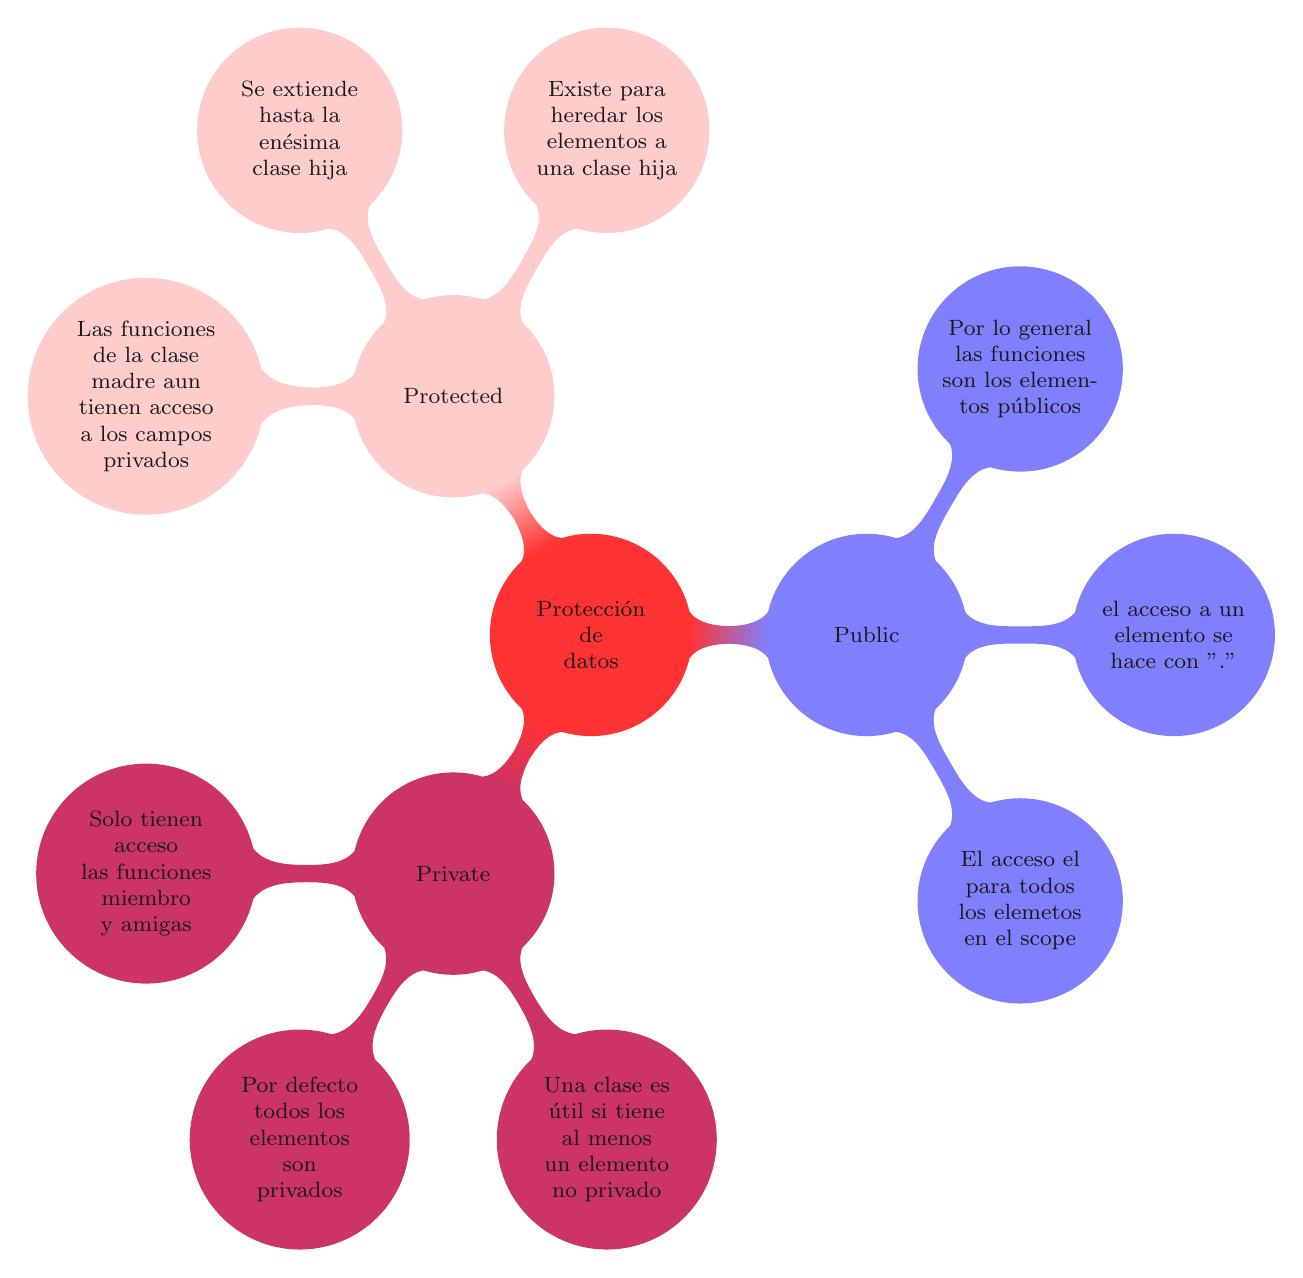
\begin{tikzpicture}[small mindmap, grow cyclic, every node/.style=concept, concept color=red!80, text=black!90, minimum size=2.5cm,
    level 1/.style={level distance=2.0cm,sibling angle=360/4},
    level 1/.style={level distance=3.5cm,sibling angle=360/3},
    level 2/.style={level distance=3.9cm,sibling angle=60},
    level 3/.style={level distance=3.5cm,sibling angle=60},
    ]

    \node{Protección\\de\\datos}
    child[concept color=purple!80] { node {Private}
        child { node {Solo tienen acceso\\las funciones miembro y amigas} }
        child { node {Por defecto todos los elementos\\son\\privados} }
        child { node {Una clase es útil si tiene al menos un elemento no privado} }
    }
    child[concept color=blue!50] { node {Public}
        child { node {El acceso el para todos los elemetos en el scope} }
        child { node {el acceso a un elemento se hace con "."} }
        child { node {Por lo general las funciones son los elementos públicos} }
    }
    child[concept color=pink!80] { node {Protected}
        child { node {Existe para heredar los elementos a una clase hija} }
        child { node {Se extiende hasta la enésima clase hija} }
        child { node {Las funciones de la clase madre aun tienen acceso a los campos privados} }
    }

    ;
\end{tikzpicture}
\end{center}
\end{document}


